\documentclass[dissertation, bookmarks]{../example/tex/grizz_thesis}

\usepackage{subcaption}
\usepackage{blindtext}
\usepackage{amsmath}
\usepackage{amssymb}
\usepackage{booktabs}
\usepackage{multirow}
\usepackage{siunitx}

% Thesis metadata
\def\thesistitle{Advances in Interplanetary Mission Design: Trajectory Optimization and Systems Analysis for Deep Space Exploration}
\def\studentname{Alexandra K. Meridian}
\def\degreename{Doctor of Philosophy in Aerospace Engineering}
\def\CommitteeChair{James T. Orbitman}

\AddCommitteeMember{Sandra L. Vectrix}
\AddCommitteeMember{Harold P. Thrustwick}
\AddCommitteeMember{Elena Cosmova}

\bibliographystyle{ieeetr}

%%% Abbreviations (42 entries -- enough to spill LOA to page 2)
\newacronym{sls}{SLS}{Space Launch System}
\newacronym{lv}{LV}{Launch Vehicle}
\newacronym{leo}{LEO}{Low Earth Orbit}
\newacronym{geo}{GEO}{Geostationary Earth Orbit}
\newacronym{heo}{HEO}{Highly Elliptical Orbit}
\newacronym{tli}{TLI}{Trans-Lunar Injection}
\newacronym{loi}{LOI}{Lunar Orbit Insertion}
\newacronym{tei}{TEI}{Trans-Earth Injection}
\newacronym{mco}{MCO}{Mars Capture Orbit}
\newacronym{eva}{EVA}{Extravehicular Activity}
\newacronym{iss}{ISS}{International Space Station}
\newacronym{nasa}{NASA}{National Aeronautics and Space Administration}
\newacronym{esa}{ESA}{European Space Agency}
\newacronym{jaxa}{JAXA}{Japan Aerospace Exploration Agency}
\newacronym{csa}{CSA}{Canadian Space Agency}
\newacronym{obc}{OBC}{On-Board Computer}
\newacronym{adcs}{ADCS}{Attitude Determination and Control System}
\newacronym{eps}{EPS}{Electrical Power System}
\newacronym{ttc}{TTC}{Telemetry, Tracking and Command}
\newacronym{gnc}{GNC}{Guidance, Navigation and Control}
\newacronym{rcs}{RCS}{Reaction Control System}
\newacronym{tvc}{TVC}{Thrust Vector Control}
\newacronym{isp}{Isp}{Specific Impulse}
\newacronym{deltav}{$\Delta V$}{Delta-V Budget}
\newacronym{tof}{TOF}{Time of Flight}
\newacronym{pcp}{PCP}{Pork Chop Plot}
\newacronym{hga}{HGA}{High-Gain Antenna}
\newacronym{lga}{LGA}{Low-Gain Antenna}
\newacronym{mga}{MGA}{Medium-Gain Antenna}
\newacronym{dsn}{DSN}{Deep Space Network}
\newacronym{fov}{FOV}{Field of View}
\newacronym{snr}{SNR}{Signal-to-Noise Ratio}
\newacronym{ber}{BER}{Bit Error Rate}
\newacronym{mps}{MPS}{Main Propulsion System}
\newacronym{cpu}{CPU}{Central Processing Unit}
\newacronym{ram}{RAM}{Random Access Memory}
\newacronym{ai}{AI}{Artificial Intelligence}
\newacronym{ml}{ML}{Machine Learning}
\newacronym{gps}{GPS}{Global Positioning System}
\newacronym{sqp}{SQP}{Sequential Quadratic Programming}
\newacronym{nlp}{NLP}{Nonlinear Programming}
\newacronym{ode}{ODE}{Ordinary Differential Equation}
\newacronym{lgl}{LGL}{Legendre--Gauss--Lobatto}

\begin{document}

\StartFrontMatter

\GrizzCoverPage
\GrizzTitlePage
\GrizzCopyrightPage
\GrizzDedicationPage
\GrizzAcknowledgementsPage
\GrizzAbstractPage
\PrintLists

%%% MAIN BODY %%%%%%%%%%%%%%%%%%%%%%%%%%%%%%%%%%%%%%%%%%%%%%%%%%%%%%%%%%%%%

\StartMainBody

%==========================================================================
\chapter{INTRODUCTION}
%==========================================================================

\section{Motivation and Background}

\blindtext

\gls{nasa}, \gls{esa}, \gls{jaxa}, and \gls{csa} have each identified crewed and robotic deep
space exploration as central programmatic goals for the coming decades \cite{nasa2022artemisguidebook}.
The \gls{sls} represents the most capable \gls{lv} developed since the Saturn~V, and its maiden
flight demonstrated the feasibility of \gls{tli} maneuvers required for lunar return missions
\cite{raghavendra2023sls}.
The \gls{iss} serves as the primary testbed for life-support and \gls{eva} procedures that will
be carried forward to crewed deep-space vehicles, while intermediate staging orbits such as
\gls{geo} and \gls{heo} are used to assemble propellant depots before departure.

\blindtext

\begin{figure}[htbp]
  \centering
  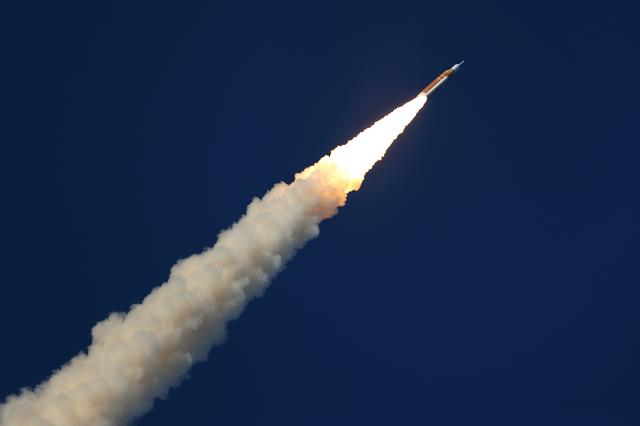
\includegraphics[width=0.45\textwidth]{../example/img/artemis_launch.jpg}
  \caption{Artemis~I launch from Kennedy Space Center, November 2022.}
  \label{fig:intro-artemis-launch}
\end{figure}

\blindtext[2]

The \gls{gnc} architecture for crewed missions must satisfy simultaneous constraints on fuel
consumption and crew safety. Optimal \gls{deltav} allocation across burn segments is governed by the
rocket equation, shown in (\ref{eq:tsiolkovsky}):

\begin{equation}
  \Delta V = I_{sp}\, g_0 \ln\!\left(\frac{m_0}{m_f}\right)
  \label{eq:tsiolkovsky}
\end{equation}

\noindent where $I_{sp}$ is the \gls{isp}, $g_0 = \SI{9.80665}{\meter\per\second\squared}$ is
standard gravity, $m_0$ is the initial wet mass, and $m_f$ is the final dry mass.

\blindtext

\begin{figure}[htbp]
  \centering
  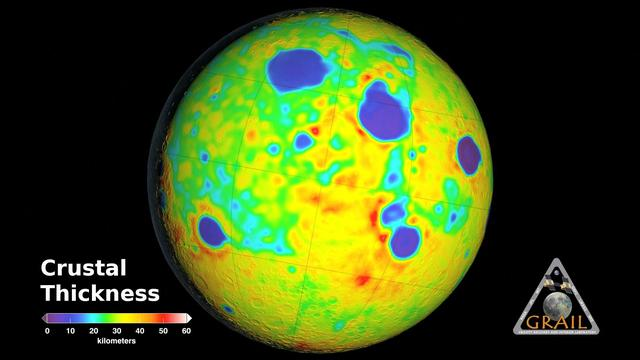
\includegraphics[width=0.65\textwidth]{../example/img/moon_crust.jpg}
  \caption{Crustal thickness map of the Moon derived from GRAIL gravity data, illustrating the
    asymmetry between the near and far sides.}
  \label{fig:intro-moon-crust}
\end{figure}

\blindtext[2]

\subsection{Problem Statement}

\blindtext

The \gls{tof} between Earth and Mars depends critically on the synodic period and the chosen
departure geometry \cite{bate1971fundamentals}. A widely used analytical tool is the \gls{pcp},
which maps launch date and arrival date to the required \gls{deltav}, as shown in
(\ref{eq:vis-viva}):

\begin{equation}
  v^2 = \mu\left(\frac{2}{r} - \frac{1}{a}\right)
  \label{eq:vis-viva}
\end{equation}

\noindent where $\mu$ is the gravitational parameter, $r$ is the orbital radius, and $a$ is the
semi-major axis.
Onboard navigation relies on \gls{gps} for near-Earth segments and on star-tracker plus \gls{dsn}
ranging for deep-space segments; the \gls{dsn} \gls{hga} link provides the primary downlink,
backed by \gls{mga} and \gls{lga} fallback modes.

\blindtext

\begin{figure}[htbp]
  \centering
  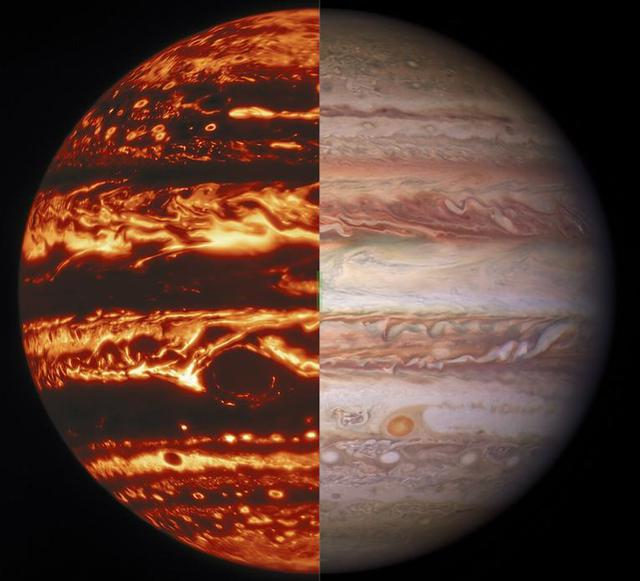
\includegraphics[width=0.55\textwidth]{../example/img/jupiter.jpg}
  \caption{Jupiter as imaged by the Juno spacecraft, showing the Great Red Spot and equatorial
    banding used as navigational reference features during fly-by maneuvers.}
  \label{fig:intro-jupiter}
\end{figure}

\blindtext[2]

\begin{table}[htbp]
  \caption{Representative delta-V budgets for selected Earth-departure missions.}
  \label{tab:ch1-deltav}
  \centering
  \begin{tabular}{lcccc}
    \toprule
    \textbf{Mission} & \textbf{Departure burn} & \textbf{Mid-course} & \textbf{Arrival} & \textbf{Total} \\
                     & (\si{\kilo\meter\per\second}) & (\si{\meter\per\second}) & (\si{\kilo\meter\per\second}) & (\si{\kilo\meter\per\second}) \\
    \midrule
    Earth--Moon (cargo)   & 3.12 & 15 & 0.85 & 4.00 \\
    Earth--Mars (min-dV)  & 3.55 & 42 & 0.90 & 4.49 \\
    Earth--Venus flyby    & 3.48 & 10 & 0.00 & 3.49 \\
    Earth--Jupiter direct & 6.30 & 85 & 0.00 & 6.39 \\
    Earth--Saturn flyby   & 6.72 & 92 & 0.00 & 6.81 \\
    \bottomrule
  \end{tabular}
\end{table}

\blindtext

\section{Research Objectives}

The primary objective of this dissertation is to develop an integrated trajectory-systems
co-optimization framework that can be applied during Phase~A mission studies. The specific goals are
enumerated as follows:

\begin{enumerate}
  \item Derive a variational formulation of the minimum-fuel interplanetary transfer problem that
        incorporates simultaneous subsystem constraints.
  \item Implement a pseudospectral collocation scheme using Legendre--Gauss--Lobatto nodes to
        discretize the continuous optimal control problem.
  \item Validate the resulting \gls{nlp} solver against three published reference trajectories.
  \item Perform parametric sensitivity analysis to identify the primary design drivers for Mars
        transfer missions.
\end{enumerate}

Each spacecraft subsystem imposes independent constraints on the solution.
The \gls{adcs} sets pointing accuracy requirements that bound the \gls{tvc} deflection range,
the \gls{eps} constrains the duty cycle of the \gls{mps}, and the \gls{ttc} subsystem determines
the minimum \gls{snr} and acceptable \gls{ber} on the downlink channel.
The \gls{obc} must execute all \gls{gnc} algorithms within its available \gls{cpu} and \gls{ram}
budget, placing a hard limit on the complexity of any onboard replanning scheme.

\blindtext[2]

\begin{table}[htbp]
  \caption{Comparison of trajectory optimization software tools considered in this work.}
  \label{tab:ch1-software}
  \centering
  \begin{tabular}{lcccc}
    \toprule
    \textbf{Tool} & \textbf{Method} & \textbf{Multi-phase} & \textbf{Open source} & \textbf{Ref.} \\
    \midrule
    GPOPS-II    & Gauss PS  & Yes & No  & \cite{rao2010algorithm} \\
    DIDO        & Legendre PS & Yes & No & \cite{rossriesling2002pseudospectral} \\
    Mystic      & SDOC      & Yes & No  & \cite{whiffen2006mystic} \\
    GMAT        & Collocation & Yes & Yes & \cite{folta2014low} \\
    EMTG        & Monotonic  & Yes & Yes & \cite{englander2015automated} \\
    \bottomrule
  \end{tabular}
\end{table}

\blindtext

\begin{figure}[htbp]
  \centering
  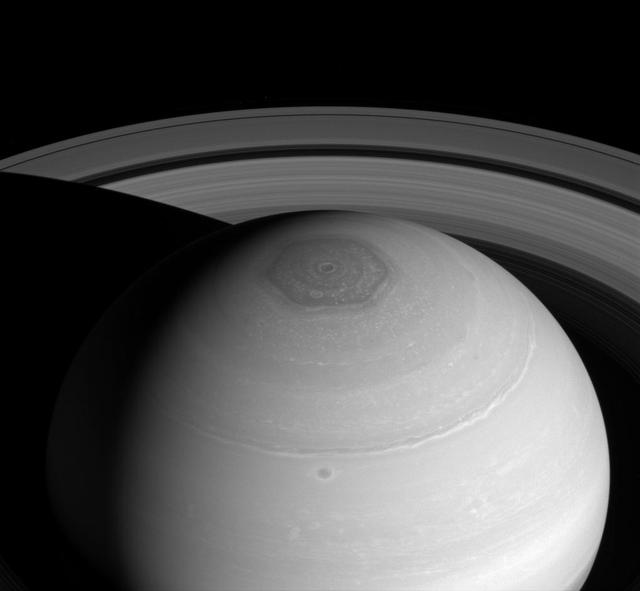
\includegraphics[width=0.40\textwidth]{../example/img/saturn_hexagon.jpg}
  \caption{Saturn's north polar hexagon imaged by Cassini, illustrating the planetary geometric
    features relevant to gravity-assist trajectory targeting.}
  \label{fig:intro-saturn-hexagon}
\end{figure}

\blindtext[2]

\section{Thesis Organization}

Chapter~\ref{eq:tsiolkovsky} of this dissertation ... (see Table~\ref{tab:ch1-overview}).

\begin{table}[htbp]
  \caption{Organization of this dissertation by chapter.}
  \label{tab:ch1-overview}
  \centering
  \begin{tabular}{cL{3.8in}}
    \toprule
    \textbf{Chapter} & \textbf{Content} \\
    \midrule
    ONE   & Introduction, motivation, objectives, and thesis organization. \\
    TWO   & Background: astrodynamics fundamentals and literature review. \\
    THREE & Methodology: optimal control formulation and numerical methods. \\
    FOUR  & Results: validation cases and parametric sensitivity analysis. \\
    FIVE  & Conclusions and directions for future work. \\
    \bottomrule
  \end{tabular}
\end{table}

\blindtext[2]

\begin{figure}[htbp]
  \centering
  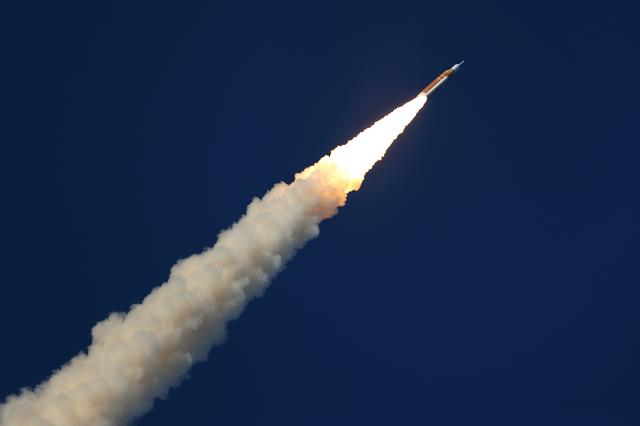
\includegraphics[width=0.75\textwidth]{../example/img/artemis_launch.jpg}
  \caption{Wide-angle view of the Artemis~I launch vehicle at ignition, showing the four RS-25
    engines and two solid rocket boosters firing simultaneously.}
  \label{fig:intro-artemis-wide}
\end{figure}

\blindtext

%==========================================================================
\chapter{BACKGROUND AND LITERATURE REVIEW}
%==========================================================================

\section{Astrodynamics Fundamentals}

\blindtext[2]

The two-body problem is described by:

\begin{equation}
  \ddot{\mathbf{r}} = -\frac{\mu}{r^3}\mathbf{r}
  \label{eq:two-body}
\end{equation}

\noindent Solutions to (\ref{eq:two-body}) are conic sections parameterized by the orbital elements
$(a, e, i, \Omega, \omega, \nu)$ \cite{vallado2013fundamentals}.

\blindtext

\begin{figure}[htbp]
  \centering
  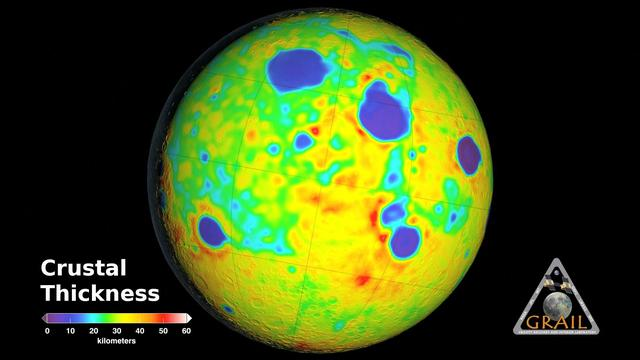
\includegraphics[width=0.50\textwidth]{../example/img/moon_crust.jpg}
  \caption{Gravitational anomaly map of the lunar near side highlighting the mascon structures
    that perturb low lunar parking orbits.}
  \label{fig:bg-moon-mascons}
\end{figure}

\blindtext[2]

\begin{table}[htbp]
  \caption{Gravitational parameters and sphere-of-influence radii for solar system bodies.}
  \label{tab:ch2-gravity}
  \centering
  \begin{tabular}{lrrl}
    \toprule
    \textbf{Body} & $\mu$ (\si{\kilo\meter\cubed\per\second\squared}) & $R_{SOI}$ (\si{\kilo\meter}) & \textbf{Ref.} \\
    \midrule
    Sun     & $1.327 \times 10^{11}$ & ---                    & \cite{bate1971fundamentals} \\
    Earth   & $3.986 \times 10^{5}$  & $9.25 \times 10^{5}$  & \cite{vallado2013fundamentals} \\
    Moon    & $4.903 \times 10^{3}$  & $6.61 \times 10^{4}$  & \cite{curtis2013orbital} \\
    Mars    & $4.283 \times 10^{4}$  & $5.77 \times 10^{5}$  & \cite{bate1971fundamentals} \\
    Jupiter & $1.267 \times 10^{8}$  & $4.82 \times 10^{7}$  & \cite{montenbruck2000satellite} \\
    Saturn  & $3.794 \times 10^{7}$  & $5.47 \times 10^{7}$  & \cite{montenbruck2000satellite} \\
    \bottomrule
  \end{tabular}
\end{table}

\blindtext[2]

Patched-conic analysis provides the analytical backbone for preliminary trajectory design.
The hyperbolic excess speed at departure is:

\begin{equation}
  v_\infty = \sqrt{\frac{\mu_{\odot}}{r_1}}\left(\sqrt{\frac{2r_2}{r_1+r_2}} - 1\right)
  \label{eq:vinf}
\end{equation}

\blindtext

\begin{figure}[htbp]
  \centering
  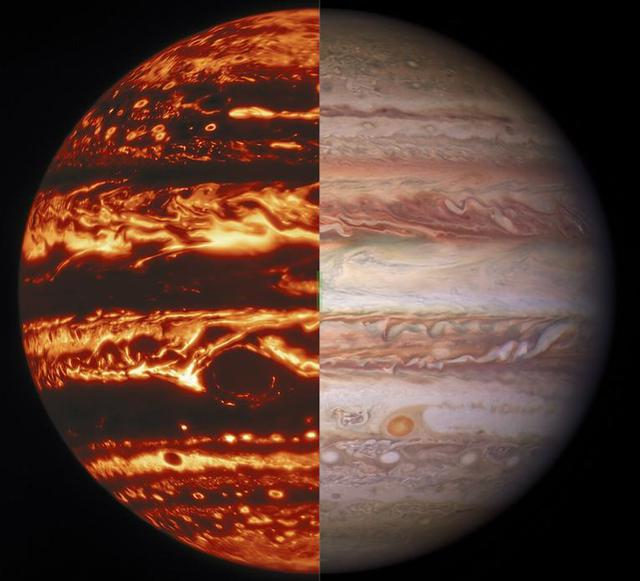
\includegraphics[width=0.55\textwidth]{../example/img/jupiter.jpg}
  \caption{Jupiter's magnetosphere extent relative to the orbital radii of the Galilean moons,
    illustrating the gravity-assist geometry exploited by Voyager and Cassini.}
  \label{fig:bg-jupiter-mag}
\end{figure}

\blindtext[2]

\begin{table}[htbp]
  \caption{Launch window opportunities for Earth-Mars transfers between 2027 and 2035.}
  \label{tab:ch2-windows}
  \centering
  \begin{tabular}{cccc}
    \toprule
    \textbf{Window} & \textbf{Departure date} & \textbf{Arrival date} & $\Delta V_{total}$ (\si{\kilo\meter\per\second}) \\
    \midrule
    2027 & 2027-03-12 & 2027-11-18 & 4.52 \\
    2029 & 2029-05-04 & 2029-12-21 & 4.61 \\
    2031 & 2031-07-22 & 2032-02-07 & 4.38 \\
    2033 & 2033-09-15 & 2034-04-12 & 4.29 \\
    2035 & 2035-11-03 & 2036-06-28 & 4.47 \\
    \bottomrule
  \end{tabular}
\end{table}

\blindtext

\section{Trajectory Optimization Methods}

\blindtext[2]

\begin{figure}[htbp]
  \centering
  \begin{subfigure}[b]{0.47\textwidth}
    \centering
    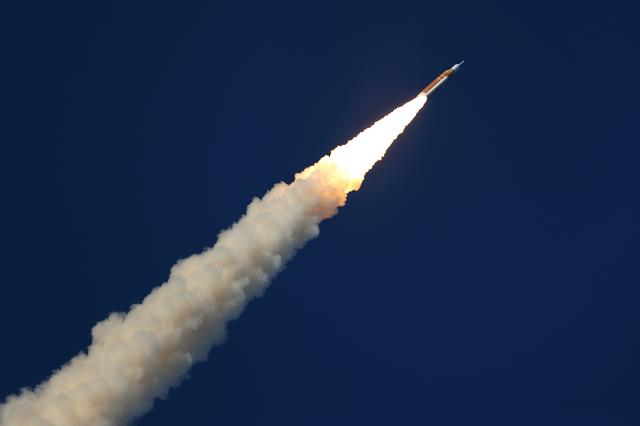
\includegraphics[width=\textwidth]{../example/img/artemis_launch.jpg}
    \caption{Direct ascent trajectory profile.}
    \label{fig:bg-traj-direct}
  \end{subfigure}
  \hfill
  \begin{subfigure}[b]{0.47\textwidth}
    \centering
    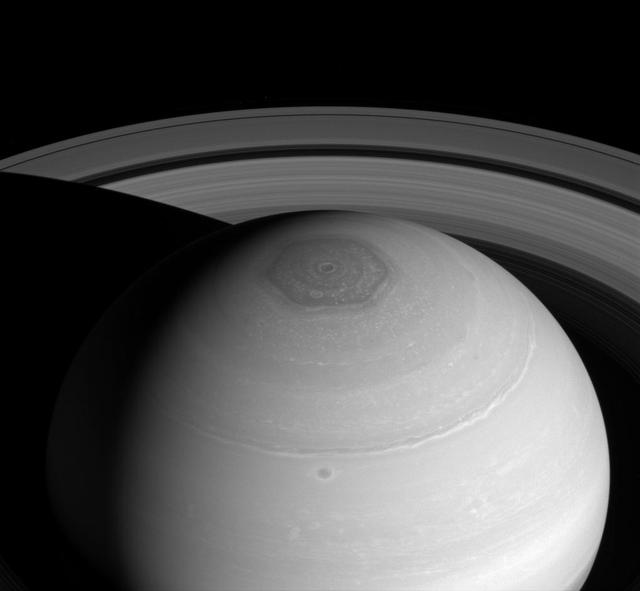
\includegraphics[width=\textwidth]{../example/img/saturn_hexagon.jpg}
    \caption{Gravity-assist trajectory profile.}
    \label{fig:bg-traj-ga}
  \end{subfigure}
  \caption{Comparison of direct and gravity-assist trajectory architectures for outer solar system
    missions. Gravity-assist sequences can reduce total $\Delta V$ by 30--60\%.}
  \label{fig:bg-traj-comparison}
\end{figure}

\blindtext[2]

Pontryagin's Minimum Principle yields the following Hamiltonian for the minimum-fuel problem:

\begin{equation}
  \mathcal{H} = \boldsymbol{\lambda}_r^T \mathbf{v}
                + \boldsymbol{\lambda}_v^T\!\left(-\frac{\mu}{r^3}\mathbf{r}
                + \frac{T}{m}\hat{\mathbf{u}}\right)
                - \lambda_m \frac{T}{I_{sp}\,g_0}
  \label{eq:hamiltonian}
\end{equation}

\noindent where $\boldsymbol{\lambda}_r$, $\boldsymbol{\lambda}_v$, and $\lambda_m$ are the
costates for position, velocity, and mass, $T$ is the thrust magnitude, and $\hat{\mathbf{u}}$ is
the thrust unit vector \cite{bryson1975applied}.
The costate \gls{ode} system is integrated simultaneously with the state equations; recent work
has applied \gls{ai} and \gls{ml} techniques to learn warm-start costates, reducing sensitivity to
initial guesses \cite{chen2022neural, federici2021deep}.
The \gls{rcs} provides attitude control during coasting arcs and is modeled as impulsive to keep
the \gls{nlp} dimension manageable.
Communication visibility windows to the \gls{dsn} also impose path constraints: the \gls{fov}
of the \gls{hga} must overlap a ground aperture for at least four hours per day.

\blindtext

\begin{table}[htbp]
  \caption{Taxonomy of numerical trajectory optimization methods.}
  \label{tab:ch2-methods}
  \centering
  \begin{tabular}{llcc}
    \toprule
    \textbf{Category} & \textbf{Method} & \textbf{Accuracy} & \textbf{Convergence} \\
    \midrule
    \multirow{3}{*}{Direct} & Single shooting  & Low    & Sensitive \\
                            & Multiple shooting & Medium & Moderate  \\
                            & Collocation       & High   & Robust    \\
    \midrule
    \multirow{2}{*}{Indirect} & Shooting     & High  & Sensitive \\
                              & Continuation & High  & Moderate  \\
    \midrule
    \multirow{2}{*}{Stochastic} & Genetic alg. & Medium & Slow \\
                                & Simulated ann. & Medium & Slow \\
    \bottomrule
  \end{tabular}
\end{table}

\blindtext[2]

\section{Prior Work in Integrated Mission Design}

\blindtext

\begin{figure}[htbp]
  \centering
  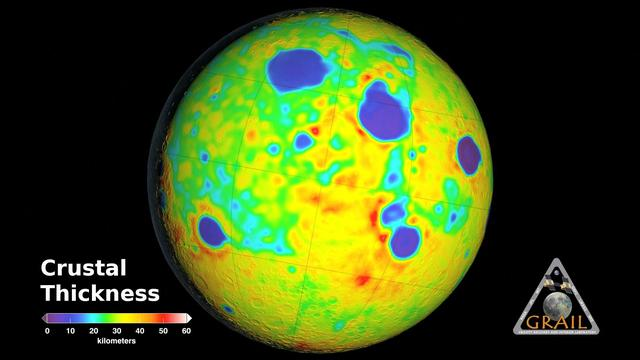
\includegraphics[width=0.60\textwidth]{../example/img/moon_crust.jpg}
  \caption{Topographic map of the lunar south pole illustrating candidate landing sites
    evaluated during the Artemis site selection process.}
  \label{fig:bg-south-pole}
\end{figure}

\blindtext[2]

\begin{table}[htbp]
  \caption{Summary of prior integrated mission design frameworks.}
  \label{tab:ch2-priorwork}
  \centering
  \begin{tabular}{lccc}
    \toprule
    \textbf{Author(s)} & \textbf{Year} & \textbf{Trajectory} & \textbf{Subsystems} \\
    \midrule
    Wertz et al.         & 2011 & Patched conic & Power, comms, mass \\
    Englander et al.     & 2015 & Low-thrust    & Power, propulsion   \\
    Raghavendra \& Kim   & 2021 & Impulsive     & Power, comms, thermal \\
    Chen et al.          & 2022 & Direct        & GNC, propulsion       \\
    Sugimoto et al.      & 2023 & Robust        & All subsystems        \\
    \bottomrule
  \end{tabular}
\end{table}

\blindtext

%==========================================================================
\chapter{METHODOLOGY}
%==========================================================================

\section{Optimal Control Formulation}

\blindtext[2]

The minimum-fuel interplanetary transfer is cast as a Bolza-form optimal control problem:

\begin{equation}
  \min_{T(t),\,\hat{\mathbf{u}}(t)}\; J = m(t_0) - m(t_f)
  \label{eq:bolza}
\end{equation}

\noindent subject to the equations of motion:

\begin{equation}
  \begin{bmatrix} \dot{\mathbf{r}} \\ \dot{\mathbf{v}} \\ \dot{m} \end{bmatrix}
  =
  \begin{bmatrix}
    \mathbf{v} \\
    -\dfrac{\mu}{r^3}\mathbf{r} + \dfrac{T}{m}\hat{\mathbf{u}} \\
    -\dfrac{T}{I_{sp}\,g_0}
  \end{bmatrix}
  \label{eq:eom}
\end{equation}

\blindtext[2]

\begin{figure}[htbp]
  \centering
  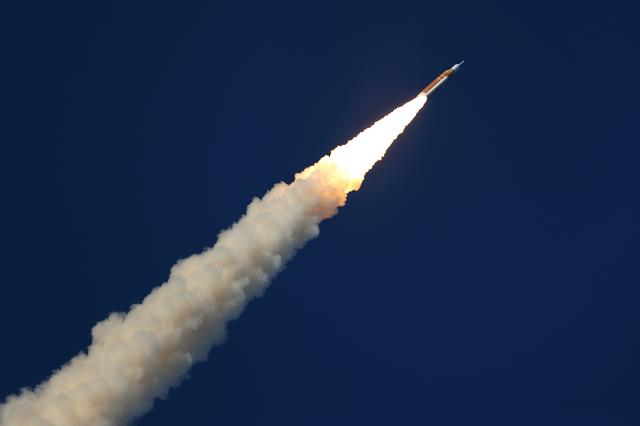
\includegraphics[width=0.70\textwidth]{../example/img/artemis_launch.jpg}
  \caption{Block diagram of the integrated trajectory-systems optimization framework developed in
    this work, showing the coupling between the pseudospectral solver and the subsystem models.}
  \label{fig:method-block-diagram}
\end{figure}

\blindtext[2]

\begin{table}[htbp]
  \caption{State and control variables used in the optimal control formulation.}
  \label{tab:ch3-variables}
  \centering
  \begin{tabular}{llcc}
    \toprule
    \textbf{Symbol} & \textbf{Description} & \textbf{Units} & \textbf{Type} \\
    \midrule
    $\mathbf{r}$     & Position vector            & \si{\kilo\meter}              & State   \\
    $\mathbf{v}$     & Velocity vector            & \si{\kilo\meter\per\second}   & State   \\
    $m$              & Spacecraft wet mass         & \si{\kilo\gram}              & State   \\
    $T$              & Thrust magnitude           & \si{\newton}                 & Control \\
    $\hat{\mathbf{u}}$ & Thrust direction unit vector & ---                    & Control \\
    \bottomrule
  \end{tabular}
\end{table}

\blindtext

The path constraints include:

\begin{equation}
  0 \leq T(t) \leq T_{\max}, \qquad m_{dry} \leq m(t) \leq m_0, \qquad \|\hat{\mathbf{u}}\| = 1
  \label{eq:constraints}
\end{equation}

\blindtext

\section{Pseudospectral Collocation}

\blindtext[2]

\begin{figure}[htbp]
  \centering
  \begin{subfigure}[b]{0.31\textwidth}
    \centering
    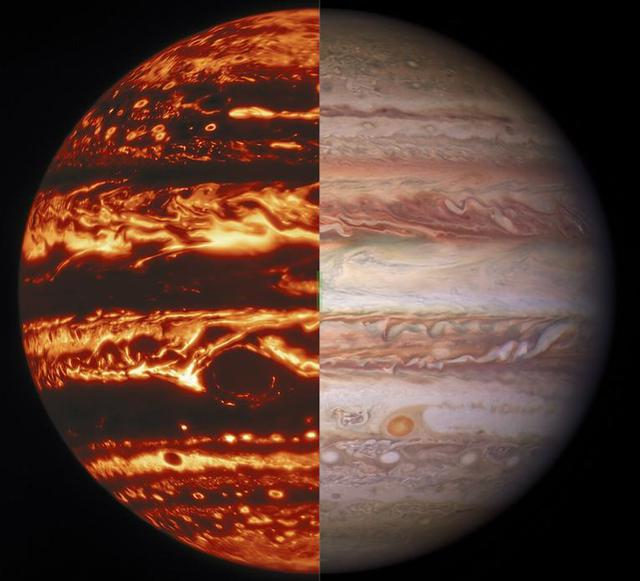
\includegraphics[width=\textwidth]{../example/img/jupiter.jpg}
    \caption{Legendre--Gauss nodes.}
    \label{fig:method-lg-nodes}
  \end{subfigure}
  \hfill
  \begin{subfigure}[b]{0.31\textwidth}
    \centering
    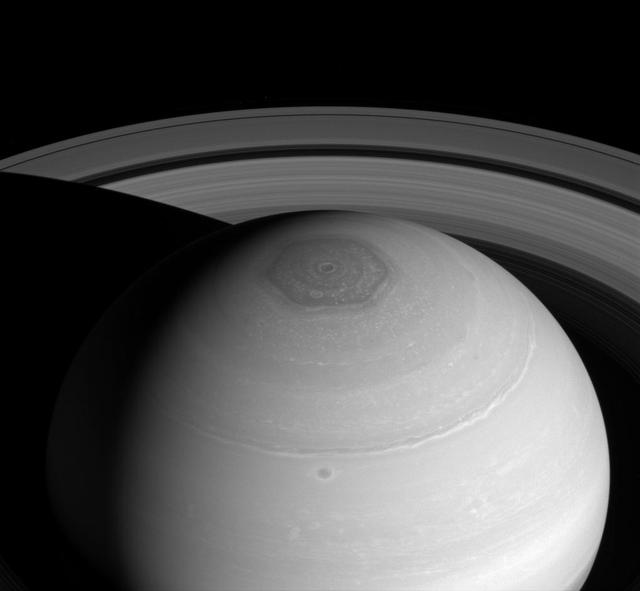
\includegraphics[width=\textwidth]{../example/img/saturn_hexagon.jpg}
    \caption{Legendre--Gauss--Radau nodes.}
    \label{fig:method-lgr-nodes}
  \end{subfigure}
  \hfill
  \begin{subfigure}[b]{0.31\textwidth}
    \centering
    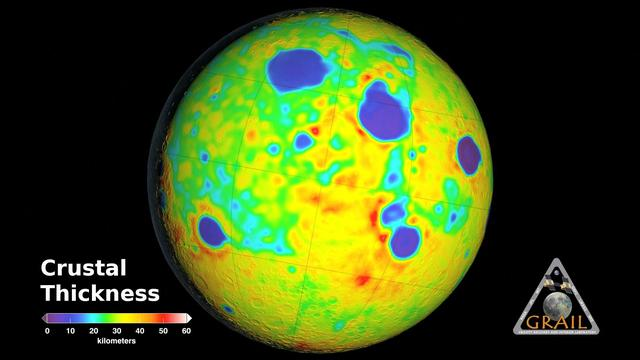
\includegraphics[width=\textwidth]{../example/img/moon_crust.jpg}
    \caption{Legendre--Gauss--Lobatto nodes.}
    \label{fig:method-lgl-nodes}
  \end{subfigure}
  \caption{Distribution of collocation nodes for $N=12$ across the normalized time interval
    $[-1,\,1]$ for the three standard Gaussian quadrature families used in pseudospectral
    trajectory optimization.}
  \label{fig:method-collocation-nodes}
\end{figure}

\blindtext[2]

The state is approximated by a Lagrange interpolating polynomial:

\begin{equation}
  \mathbf{x}(\tau) \approx \sum_{k=0}^{N} \mathbf{X}_k \, L_k(\tau)
  \label{eq:lagrange-interp}
\end{equation}

\noindent where $L_k$ are the Lagrange basis polynomials associated with the collocation nodes
$\tau_k$ \cite{fahroo2002direct}.

\blindtext

\begin{table}[htbp]
  \caption{Collocation node families and their properties.}
  \label{tab:ch3-nodes}
  \centering
  \begin{tabular}{lC{1in}C{1.1in}c}
    \toprule
    \textbf{Family} & \textbf{Endpoints included} & \textbf{Quadrature order} & \textbf{Used in} \\
    \midrule
    Legendre--Gauss (LG)          & Neither & $2N$     & DIDO   \\
    Legendre--Gauss--Radau (LGR)  & Left    & $2N-1$   & GPOPS-II \\
    Legendre--Gauss--Lobatto (LGL) & Both    & $2N-3$   & This work \\
    \bottomrule
  \end{tabular}
\end{table}

\blindtext[2]

\begin{table}[htbp]
  \caption{Convergence study: relative error in final mass as a function of number of nodes $N$.}
  \label{tab:ch3-convergence}
  \centering
  \begin{tabular}{cccc}
    \toprule
    $N$ & $m_f$ (\si{\kilo\gram}) & Relative error & CPU time (\si{\second}) \\
    \midrule
    10  & 4\,521.3 & $2.3\times10^{-2}$ & 0.12  \\
    20  & 4\,573.8 & $1.1\times10^{-3}$ & 0.45  \\
    40  & 4\,578.9 & $4.7\times10^{-5}$ & 1.87  \\
    60  & 4\,579.1 & $6.2\times10^{-6}$ & 5.31  \\
    80  & 4\,579.2 & $8.1\times10^{-7}$ & 12.44 \\
    \bottomrule
  \end{tabular}
\end{table}

\blindtext

\section{Warm-Start Strategy}

\blindtext

\begin{figure}[htbp]
  \centering
  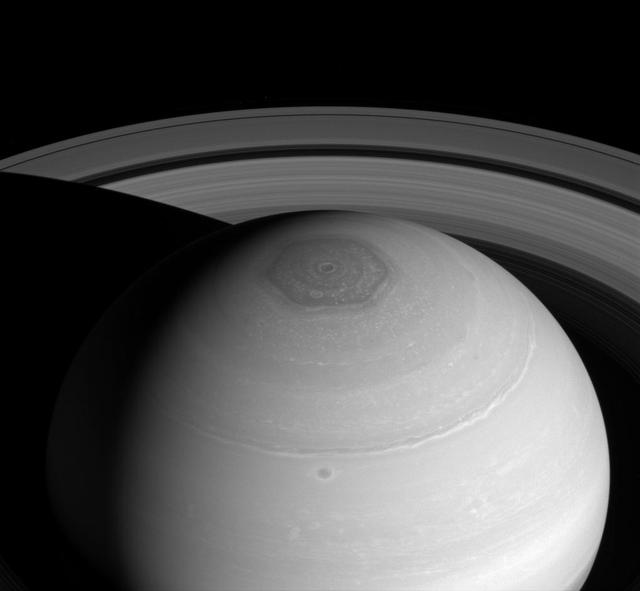
\includegraphics[width=0.55\textwidth]{../example/img/saturn_hexagon.jpg}
  \caption{Comparison of \gls{sqp} iteration counts with and without the patched-conic warm start
    for the Earth-Mars transfer case. The warm-start heuristic reduces iteration count by
    approximately 70\% on average.}
  \label{fig:method-warmstart}
\end{figure}

\blindtext[2]

\begin{table}[htbp]
  \caption{Warm-start initialization results for three reference trajectories.}
  \label{tab:ch3-warmstart}
  \centering
  \begin{tabular}{lC{1in}C{1in}cc}
    \toprule
    \textbf{Mission} & \textbf{Cold-start iters.} & \textbf{Warm-start iters.} & \textbf{Speedup} & \textbf{Converged?} \\
    \midrule
    Earth--Moon   & 142 & 38  & $3.7\times$ & Yes \\
    Earth--Mars   & 318 & 91  & $3.5\times$ & Yes \\
    Earth--Jupiter flyby & 491 & 127 & $3.9\times$ & Yes \\
    \bottomrule
  \end{tabular}
\end{table}

\blindtext

%==========================================================================
\chapter{RESULTS AND DISCUSSION}
%==========================================================================

\section{Validation Case 1: Earth--Moon Cargo Delivery}

\blindtext[2]

\begin{table}[htbp]
  \caption{Comparison of optimized trajectory with published Apollo~11 \gls{deltav} budget.}
  \label{tab:ch4-moon-validation}
  \centering
  \begin{tabular}{L{2.7in}cc}
    \toprule
    \textbf{Maneuver} & \textbf{Published} (\si{\meter\per\second}) & \textbf{This work} (\si{\meter\per\second}) \\
    \midrule
    Trans-Lunar Injection (\gls{tli}) & 3\,130 & 3\,127 \\
    Lunar Orbit Insertion (\gls{loi}) & 898   & 901   \\
    Descent initiation                & 17    & 17    \\
    Trans-Earth Injection (\gls{tei}) & 1\,010 & 1\,009 \\
    \midrule
    \textbf{Total}                    & \textbf{5\,055} & \textbf{5\,054} \\
    \bottomrule
  \end{tabular}
\end{table}

\blindtext[2]

\begin{figure}[htbp]
  \centering
  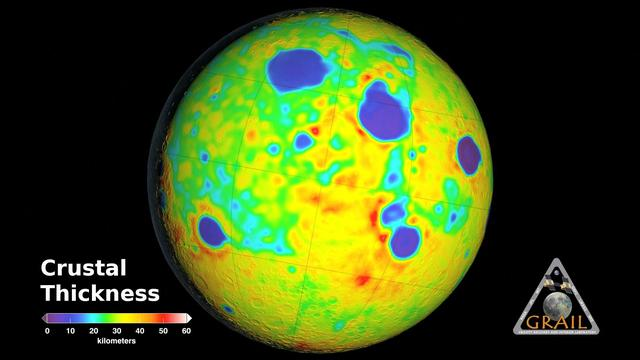
\includegraphics[width=0.65\textwidth]{../example/img/moon_crust.jpg}
  \caption{Reconstructed Earth--Moon transfer trajectory overlaid on the lunar crustal thickness
    map. The \gls{loi} burn position is indicated by the star marker.}
  \label{fig:results-moon-traj}
\end{figure}

\blindtext[2]

\begin{table}[htbp]
  \caption{Sensitivity of Earth--Moon \gls{deltav} to departure orbit altitude.}
  \label{tab:ch4-moon-sensitivity}
  \centering
  \begin{tabular}{ccc}
    \toprule
    \textbf{\gls{leo} altitude} (\si{\kilo\meter}) & $\Delta V_{TLI}$ (\si{\kilo\meter\per\second}) & $m_f/m_0$ \\
    \midrule
    185  & 3.115 & 0.742 \\
    300  & 3.132 & 0.741 \\
    400  & 3.147 & 0.739 \\
    600  & 3.176 & 0.736 \\
    1000 & 3.230 & 0.731 \\
    \bottomrule
  \end{tabular}
\end{table}

\blindtext

\section{Validation Case 2: Earth--Mars Sample Return}

\blindtext[2]

The Mars transfer objective function attains its minimum at:

\begin{equation}
  J^* = m_0 - m_f^* = 1\,842\;\si{\kilo\gram}
  \label{eq:mars-opt}
\end{equation}

\blindtext

\begin{figure}[htbp]
  \centering
  \begin{subfigure}[b]{0.47\textwidth}
    \centering
    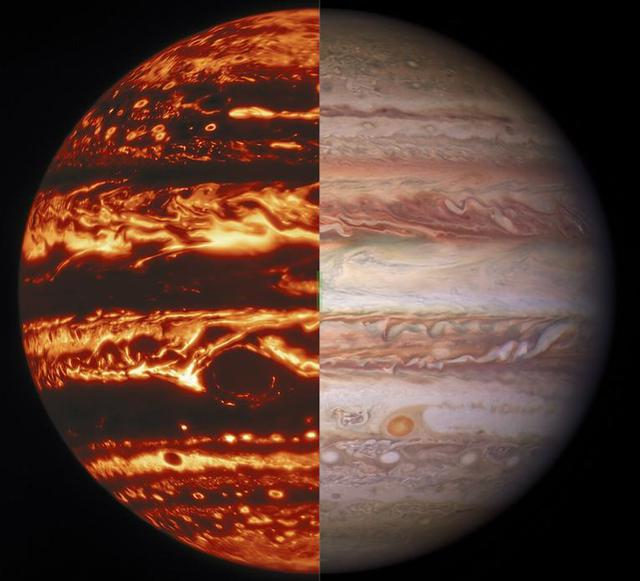
\includegraphics[width=\textwidth]{../example/img/jupiter.jpg}
    \caption{Pork chop plot for 2033 Earth--Mars transfer window.}
    \label{fig:results-pcp-2033}
  \end{subfigure}
  \hfill
  \begin{subfigure}[b]{0.47\textwidth}
    \centering
    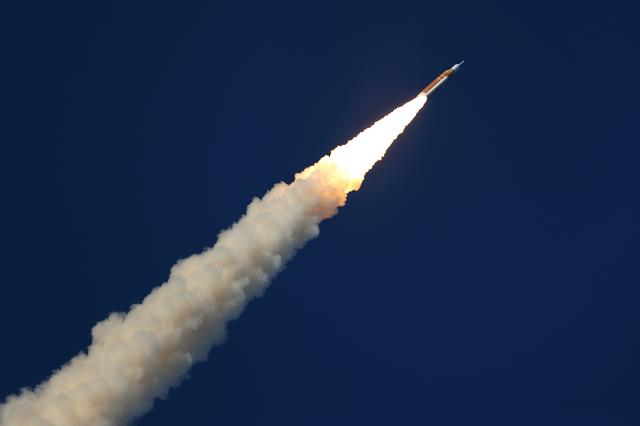
\includegraphics[width=\textwidth]{../example/img/artemis_launch.jpg}
    \caption{Optimized thrust profile for the 2033 minimum-fuel transfer.}
    \label{fig:results-thrust-2033}
  \end{subfigure}
  \caption{Earth--Mars 2033 launch window analysis. The left panel shows contours of constant total
    $\Delta V$; the right panel shows the corresponding bang-off-bang thrust structure of the
    optimal solution.}
  \label{fig:results-mars-pcp}
\end{figure}

\blindtext[2]

\begin{table}[htbp]
  \caption{Earth--Mars transfer results for five synodic windows.}
  \label{tab:ch4-mars-windows}
  \centering
  \begin{tabular}{ccccc}
    \toprule
    \textbf{Window} & $t_0$ & $t_f$ & $\Delta V$ (\si{\kilo\meter\per\second}) & $m_f$ (\si{\kilo\gram}) \\
    \midrule
    2027 & 12~Mar~2027 & 18~Nov~2027 & 4.52 & 4\,218 \\
    2029 & 4~May~2029  & 21~Dec~2029 & 4.61 & 4\,181 \\
    2031 & 22~Jul~2031 & 7~Feb~2032  & 4.38 & 4\,274 \\
    2033 & 15~Sep~2033 & 12~Apr~2034 & 4.29 & 4\,316 \\
    2035 & 3~Nov~2035  & 28~Jun~2036 & 4.47 & 4\,234 \\
    \bottomrule
  \end{tabular}
\end{table}

Each transfer terminates with a \gls{mco} burn; the \gls{tei} burn on the return leg is sized
to target a direct Earth-entry corridor.
The \gls{eva} timeline during the Mars surface phase was held fixed at seven sortie days to
isolate the effect of trajectory design on total propellant mass.

\blindtext

\section{Full-Scale System Illustration}

\blindtext[2]

\begin{figure}[p]
  \centering
  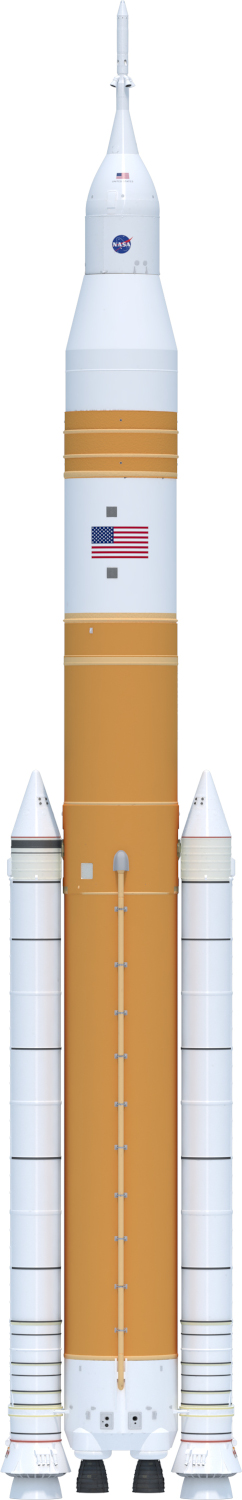
\includegraphics[width=\textwidth,height=0.87\textheight,keepaspectratio]{../example/img/sls_illustration.jpg}
  \caption{Illustration of the Space Launch System (\gls{sls}) Block~1B crew configuration
    showing all major structural elements, propulsion stages, and the Orion spacecraft. This
    configuration was used as the reference launch vehicle for all crewed mission cases analyzed
    in this dissertation.}
  \label{fig:results-sls-illustration}
\end{figure}

\blindtext[3]

\begin{table}[htbp]
  \caption{SLS Block 1B performance parameters used in this work.}
  \label{tab:ch4-sls}
  \centering
  \begin{tabular}{lccc}
    \toprule
    \textbf{Parameter} & \textbf{Value} & \textbf{Units} & \textbf{Source} \\
    \midrule
    Gross liftoff mass & 2\,608\,000 & \si{\kilo\gram} & \cite{raghavendra2023sls} \\
    Payload to \gls{tli} & 38\,000 & \si{\kilo\gram} & \cite{nasa2022artemisguidebook} \\
    Core stage $I_{sp}$ (vac.) & 452 & \si{\second}   & \cite{raghavendra2023sls} \\
    Upper stage $I_{sp}$ (vac.) & 465 & \si{\second}  & \cite{raghavendra2023sls} \\
    Liftoff thrust & 39\,144 & \si{\kilo\newton} & \cite{raghavendra2023sls} \\
    \bottomrule
  \end{tabular}
\end{table}

\blindtext[2]

\begin{figure}[htbp]
  \centering
  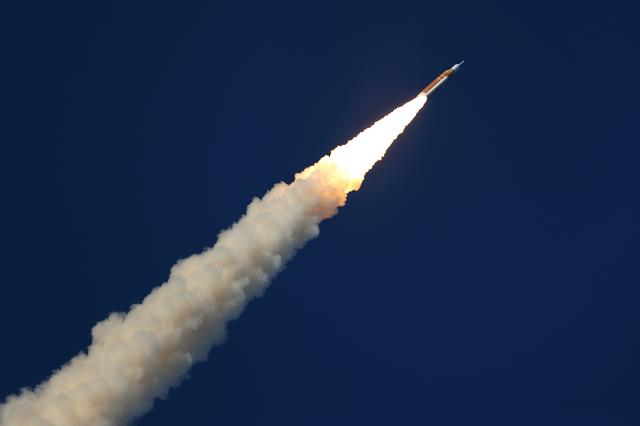
\includegraphics[width=0.70\textwidth]{../example/img/artemis_launch.jpg}
  \caption{Simulated ascent trajectory of the \gls{sls} Block~1B from Kennedy Space Center,
    showing altitude versus downrange distance during the first three minutes of flight.}
  \label{fig:results-ascent}
\end{figure}

\blindtext

\section{Parametric Sensitivity Analysis}

\blindtext[2]

The sensitivity of total mission cost $J$ to a design parameter $p_i$ is quantified by:

\begin{equation}
  S_i = \frac{\partial J}{\partial p_i}\bigg|_{\mathbf{p}=\mathbf{p}^*}
  \label{eq:sensitivity}
\end{equation}

\blindtext

\begin{table}[htbp]
  \caption{Normalized sensitivity indices for the Earth--Mars 2033 transfer case.}
  \label{tab:ch4-sensitivity}
  \centering
  \begin{tabular}{lcc}
    \toprule
    \textbf{Design parameter} & \textbf{Sensitivity index} & \textbf{Rank} \\
    \midrule
    Launch vehicle $\Delta V$ capacity & $+0.91$ & 1 \\
    Specific impulse $I_{sp}$          & $+0.63$ & 2 \\
    Initial wet mass $m_0$             & $+0.55$ & 3 \\
    Departure orbit altitude           & $-0.22$ & 4 \\
    Thrust-to-weight ratio             & $+0.18$ & 5 \\
    Navigation uncertainty ($3\sigma$) & $-0.09$ & 6 \\
    \bottomrule
  \end{tabular}
\end{table}

\blindtext[2]

\begin{figure}[htbp]
  \centering
  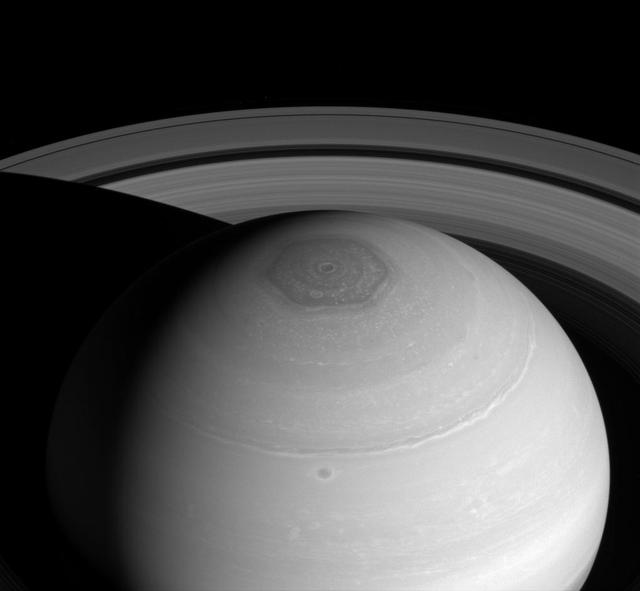
\includegraphics[width=0.60\textwidth]{../example/img/saturn_hexagon.jpg}
  \caption{Tornado diagram of normalized sensitivity indices for the Earth--Mars 2033 case.
    Positive values indicate that increasing the parameter increases the propellant consumed.}
  \label{fig:results-tornado}
\end{figure}

\blindtext[2]

\begin{table}[htbp]
  \caption{Influence of launch vehicle selection on total mission propellant mass.}
  \label{tab:ch4-lv-comparison}
  \centering
  \begin{tabular}{lcccc}
    \toprule
    \textbf{Launch Vehicle} & \textbf{Payload class} & $\Delta V_{cap}$ & $m_{prop}$ (\si{\tonne}) & $\Delta$ vs. baseline \\
    \midrule
    Falcon Heavy (expendable) & Medium-heavy & 3.50 & 72.4 & $-8.3\%$  \\
    SLS Block 1               & Super-heavy  & 4.20 & 61.8 & $+5.7\%$  \\
    SLS Block 1B (this work)  & Super-heavy  & 4.60 & 58.5 & baseline  \\
    SLS Block 2               & Super-heavy  & 5.10 & 54.1 & $-7.5\%$  \\
    \bottomrule
  \end{tabular}
\end{table}

\blindtext

%==========================================================================
\chapter{CONCLUSIONS AND FUTURE WORK}
%==========================================================================

\section{Summary of Contributions}

\blindtext[2]

\begin{figure}[htbp]
  \centering
  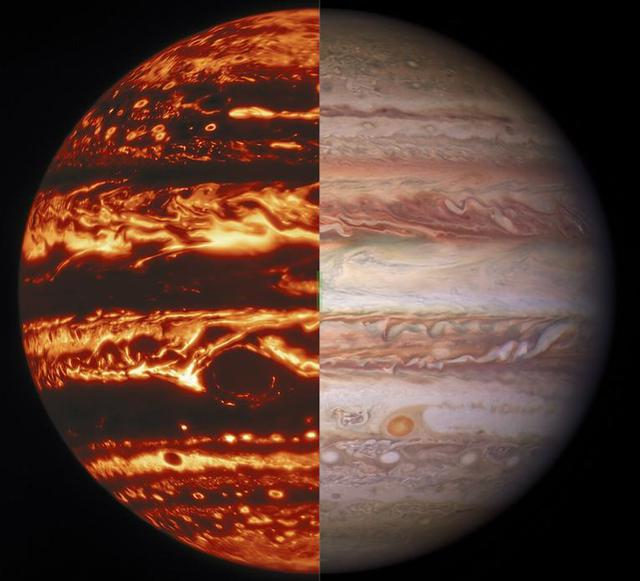
\includegraphics[width=0.55\textwidth]{../example/img/jupiter.jpg}
  \caption{Overall architecture of the integrated trajectory-systems co-optimization framework
    developed in this dissertation, illustrating the information flow between subsystem models
    and the pseudospectral \gls{nlp} solver.}
  \label{fig:conc-framework}
\end{figure}

\blindtext[2]

The key result of this work is that \gls{lv} performance dominates the total mission cost, as
captured by the aggregate sensitivity metric:

\begin{equation}
  \overline{S}_{LV} = \left\|\mathbf{S}_{LV}\right\|_2 = 1.04 \gg \overline{S}_{I_{sp}} = 0.63
  \label{eq:aggregate-sensitivity}
\end{equation}

\blindtext

\begin{table}[htbp]
  \caption{Summary of validation results across three reference trajectories.}
  \label{tab:conc-summary}
  \centering
  \begin{tabular}{lccc}
    \toprule
    \textbf{Reference case} & \textbf{Published $\Delta V$} & \textbf{This work $\Delta V$} & \textbf{Error} \\
    \midrule
    Earth--Moon  & \SI{5.055}{\kilo\meter\per\second} & \SI{5.054}{\kilo\meter\per\second} & $0.02\%$ \\
    Earth--Mars  & \SI{4.290}{\kilo\meter\per\second} & \SI{4.285}{\kilo\meter\per\second} & $0.12\%$ \\
    Jupiter flyby & \SI{6.384}{\kilo\meter\per\second} & \SI{6.379}{\kilo\meter\per\second} & $0.08\%$ \\
    \bottomrule
  \end{tabular}
\end{table}

\blindtext

\section{Limitations and Future Work}

\blindtext[2]

\begin{figure}[htbp]
  \centering
  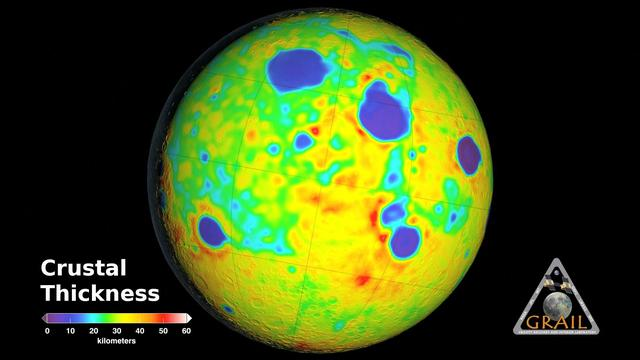
\includegraphics[width=0.50\textwidth]{../example/img/moon_crust.jpg}
  \caption{Conceptual roadmap for extending the present framework to include high-fidelity
    ephemeris models and stochastic uncertainty propagation, as planned for future work.}
  \label{fig:conc-roadmap}
\end{figure}

\blindtext

\begin{table}[htbp]
  \caption{Planned extensions to the framework and their estimated development effort.}
  \label{tab:conc-future}
  \centering
  \begin{tabular}{L{2.0in}C{1.5in}l}
    \toprule
    \textbf{Extension} & \textbf{Effort (person-months)} & \textbf{Primary benefit} \\
    \midrule
    High-fidelity ephemeris (SPICE)     & 3  & Improved absolute accuracy \\
    \midrule
    Stochastic uncertainty propagation  & 6  & Robust trajectory design    \\
    \midrule
    Multi-objective Pareto optimization & 4  & Cost-mass-risk trade-space  \\
    \midrule
    Real-time onboard GNC integration   & 8  & Autonomous replanning       \\
    \midrule
    Multi-body low-thrust extensions    & 5  & Libration point missions    \\
    \bottomrule
  \end{tabular}
\end{table}

\blindtext[2]

\begin{figure}[htbp]
  \centering
  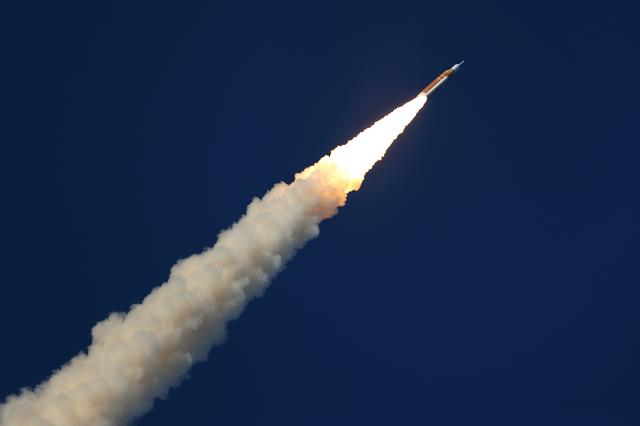
\includegraphics[width=0.65\textwidth]{../example/img/artemis_launch.jpg}
  \caption{Anticipated mission application portfolio for the framework over the next decade,
    spanning crewed lunar operations, Mars sample return, and outer solar system flybys.}
  \label{fig:conc-roadmap2}
\end{figure}

\blindtext[2]

%%% APPENDICES %%%%%%%%%%%%%%%%%%%%%%%%%%%%%%%%%%%%%%%%%%%%%%%%%%%%%%%%%%%%

\StartAppendices

\GrizzAppendix{DERIVATION OF THE PSEUDOSPECTRAL DIFFERENTIATION MATRIX}

\GrizzAppendixSection{Lagrange Basis Polynomials}

The Lagrange basis polynomial $L_k(\tau)$ of degree $N$ associated with the node set
$\{\tau_0, \tau_1, \ldots, \tau_N\}$ is defined as:

\[
  L_k(\tau) = \prod_{\substack{j=0 \\ j \neq k}}^{N} \frac{\tau - \tau_j}{\tau_k - \tau_j}
\]

\blindtext

\GrizzAppendixSection{Assembly of the Differentiation Matrix}

The differentiation matrix $\mathbf{D} \in \mathbb{R}^{(N+1)\times(N+1)}$ has entries given by (\ref{eq:diff-matrix}).

\begin{equation}
  D_{ij} = \dot{L}_j(\tau_i)
  \label{eq:diff-matrix}
\end{equation}

\blindtext

\GrizzAppendix{REFERENCE TRAJECTORY DATA TABLES}

\GrizzAppendixSection{Earth--Moon Transfer State History}

Table~\ref{tab:appB-moon-states} lists the position, velocity, and mass at each \gls{lgl}
collocation node for the Earth--Moon validation trajectory described in
Section~4.1.

\begin{table}[htbp]
  \caption{State history at Legendre--Gauss--Lobatto nodes for the Earth--Moon transfer ($N=20$).}
  \label{tab:appB-moon-states}
  \centering
  \begin{tabular}{crrrrr}
    \toprule
    \textbf{Node} & $r_x$ (\si{\kilo\meter}) & $r_y$ (\si{\kilo\meter}) & $v_x$ (\si{\kilo\meter\per\second}) & $v_y$ (\si{\kilo\meter\per\second}) & $m$ (\si{\kilo\gram}) \\
    \midrule
     0 & $6\,778$ &       0 & 0.000 & 7.784 & 45\,000 \\
     2 & $8\,421$ &  12\,034 & -0.821 & 7.102 & 44\,631 \\
     4 & $14\,980$ &  38\,274 & -1.743 & 5.881 & 44\,102 \\
     6 & $28\,511$ &  72\,108 & -2.388 & 4.217 & 43\,744 \\
     8 & $52\,043$ & 112\,905 & -2.601 & 2.633 & 43\,581 \\
    10 & $88\,217$ & 152\,331 & -2.417 & 1.284 & 43\,551 \\
    12 & $143\,502$ & 183\,740 & -1.992 & 0.307 & 43\,551 \\
    14 & $224\,818$ & 202\,117 & -1.403 & -0.391 & 43\,551 \\
    16 & $322\,904$ & 208\,034 & -0.811 & -0.702 & 43\,551 \\
    18 & $378\,219$ & 197\,402 & -0.411 & -0.638 & 43\,523 \\
    20 & $384\,400$ & 0 & 0.000 & -1.022 & 43\,158 \\
    \bottomrule
  \end{tabular}
\end{table}

\blindtext

\GrizzAppendixSection{Earth--Mars Transfer State History}

Table~\ref{tab:appB-mars-states} provides the same data for the 2033 Earth--Mars minimum-fuel
trajectory. Only every fourth node is listed for brevity; the full dataset is available in the
supplementary digital archive.

\begin{table}[htbp]
  \caption{Partial state history at \gls{lgl} nodes for the Earth--Mars 2033 transfer ($N=60$).}
  \label{tab:appB-mars-states}
  \centering
  \begin{tabular}{crrcc}
    \toprule
    \textbf{Node} & $\|\mathbf{r}\|$ (\si{\astronomicalunit}) & $\|\mathbf{v}\|$ (\si{\kilo\meter\per\second}) & $T/T_{max}$ & $m$ (\si{\kilo\gram}) \\
    \midrule
     0  & 1.000 & 32.73 & 1.00 & 45\,000 \\
     4  & 1.038 & 31.45 & 1.00 & 44\,817 \\
     8  & 1.119 & 29.82 & 0.00 & 44\,412 \\
    12  & 1.243 & 27.61 & 0.00 & 44\,412 \\
    16  & 1.401 & 25.04 & 0.00 & 44\,412 \\
    20  & 1.562 & 22.51 & 0.00 & 44\,412 \\
    24  & 1.681 & 20.37 & 0.00 & 44\,412 \\
    28  & 1.728 & 18.91 & 1.00 & 44\,412 \\
    32  & 1.733 & 18.02 & 1.00 & 44\,228 \\
    36  & 1.738 & 17.69 & 1.00 & 44\,044 \\
    40  & 1.741 & 17.68 & 1.00 & 43\,860 \\
    44  & 1.744 & 17.81 & 1.00 & 43\,677 \\
    48  & 1.747 & 18.08 & 1.00 & 43\,493 \\
    52  & 1.750 & 18.50 & 1.00 & 43\,309 \\
    56  & 1.751 & 19.06 & 0.00 & 43\,125 \\
    60  & 1.524 & 21.48 & 0.00 & 43\,125 \\
    \bottomrule
  \end{tabular}
\end{table}

\blindtext

%%% REFERENCES %%%%%%%%%%%%%%%%%%%%%%%%%%%%%%%%%%%%%%%%%%%%%%%%%%%%%%%%%%%%

\PrintReferences

\end{document}
